% Options for packages loaded elsewhere
\PassOptionsToPackage{unicode}{hyperref}
\PassOptionsToPackage{hyphens}{url}
%
\documentclass[
]{article}
\title{Applied Statistical Programming - Spring 2022}
\author{}
\date{\vspace{-2.5em}}

\usepackage{amsmath,amssymb}
\usepackage{lmodern}
\usepackage{iftex}
\ifPDFTeX
  \usepackage[T1]{fontenc}
  \usepackage[utf8]{inputenc}
  \usepackage{textcomp} % provide euro and other symbols
\else % if luatex or xetex
  \usepackage{unicode-math}
  \defaultfontfeatures{Scale=MatchLowercase}
  \defaultfontfeatures[\rmfamily]{Ligatures=TeX,Scale=1}
\fi
% Use upquote if available, for straight quotes in verbatim environments
\IfFileExists{upquote.sty}{\usepackage{upquote}}{}
\IfFileExists{microtype.sty}{% use microtype if available
  \usepackage[]{microtype}
  \UseMicrotypeSet[protrusion]{basicmath} % disable protrusion for tt fonts
}{}
\makeatletter
\@ifundefined{KOMAClassName}{% if non-KOMA class
  \IfFileExists{parskip.sty}{%
    \usepackage{parskip}
  }{% else
    \setlength{\parindent}{0pt}
    \setlength{\parskip}{6pt plus 2pt minus 1pt}}
}{% if KOMA class
  \KOMAoptions{parskip=half}}
\makeatother
\usepackage{xcolor}
\IfFileExists{xurl.sty}{\usepackage{xurl}}{} % add URL line breaks if available
\IfFileExists{bookmark.sty}{\usepackage{bookmark}}{\usepackage{hyperref}}
\hypersetup{
  pdftitle={Applied Statistical Programming - Spring 2022},
  hidelinks,
  pdfcreator={LaTeX via pandoc}}
\urlstyle{same} % disable monospaced font for URLs
\usepackage[margin=1in]{geometry}
\usepackage{graphicx}
\makeatletter
\def\maxwidth{\ifdim\Gin@nat@width>\linewidth\linewidth\else\Gin@nat@width\fi}
\def\maxheight{\ifdim\Gin@nat@height>\textheight\textheight\else\Gin@nat@height\fi}
\makeatother
% Scale images if necessary, so that they will not overflow the page
% margins by default, and it is still possible to overwrite the defaults
% using explicit options in \includegraphics[width, height, ...]{}
\setkeys{Gin}{width=\maxwidth,height=\maxheight,keepaspectratio}
% Set default figure placement to htbp
\makeatletter
\def\fps@figure{htbp}
\makeatother
\setlength{\emergencystretch}{3em} % prevent overfull lines
\providecommand{\tightlist}{%
  \setlength{\itemsep}{0pt}\setlength{\parskip}{0pt}}
\setcounter{secnumdepth}{-\maxdimen} % remove section numbering
\ifLuaTeX
  \usepackage{selnolig}  % disable illegal ligatures
\fi

\begin{document}
\maketitle

\section*{Instructions}
\begin{enumerate}
  \item The following questions should each be answered within an Rmarkdown file. Be sure to provide many comments in your code blocks to facilitate grading. Undocumented code will not be graded.
  \item Work on git. Continue to work in the repository you forked from \url{https://github.com/johnsontr/AppliedStatisticalProgramming2022} and add your code for Problem Set 5. Commit and push frequently. Use meaningful commit messages because these will affect your grade.
  \item You may work in teams, but each student should develop their own Rmarkdown file. To be clear, there should be no copy and paste. Each keystroke in the assignment should be your own.
\end{enumerate}

\section*{Numerical Integration}

Approximating an integral is a necessary part of Bayesian statistics.
Numerical integration is inherent to Monte Carlo integration, rejection
and importance sampling, Markov chain Monte Carlo, and many other
methods. Two common approximations for integration are based on the
trapezoidal rule and Simpson's rule. In this exercise, you will create
an \texttt{S4} package that performs numerical integration using these
two rules. Read the following two subsections about these
approximations, then follow the instructions to create the package.

\subsection*{Trapezoidal Rule}

Trapezoid rule is a technique for approximating the definite integral,
and it follows the mathematical expression below: \begin{align*} 
 \int_a^b f(x) dx &\approx T\\
T &= \frac{h}{2}(f(x_0) + 2f(x_1) + ... + 2(f_{n-1}) + f(x_n))\\
\text{where } h &= \frac{b-a}{n} 
\end{align*}

\begin{figure}[h!]\centering 
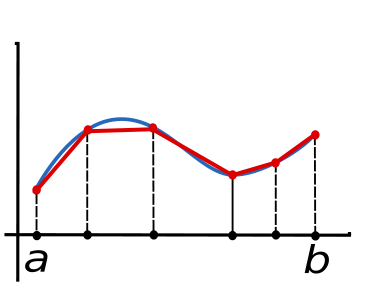
\includegraphics[width=0.6\linewidth]{trapezoidal_rule_illustration.png} 
\end{figure}

\subsection*{Simpsons Rule}

Simpson's rule is another technique for approximating a definite
integrals, numerically. It follows the approximation below:
\begin{align*} 
 \int_a^b f(x) dx &\approx S\\
S &= \frac{h}{3}(f(x_0) + 4f(x_1) + 2f(x_2) + 4f(x_3) +  ... + 4(f_{n-1}) + f(x_n))\\
\text{where } h &= \frac{b-a}{h} 
\end{align*} Image that you are drawing a parabola from the points
\((a, f(a))\) to \((b, f(b))\) that also goes through the \((m, f(m))\).
We can approximate the area under the parabola as being equal to
\(\int_a^b f(x) dx\).

\begin{figure}[h!]\centering 
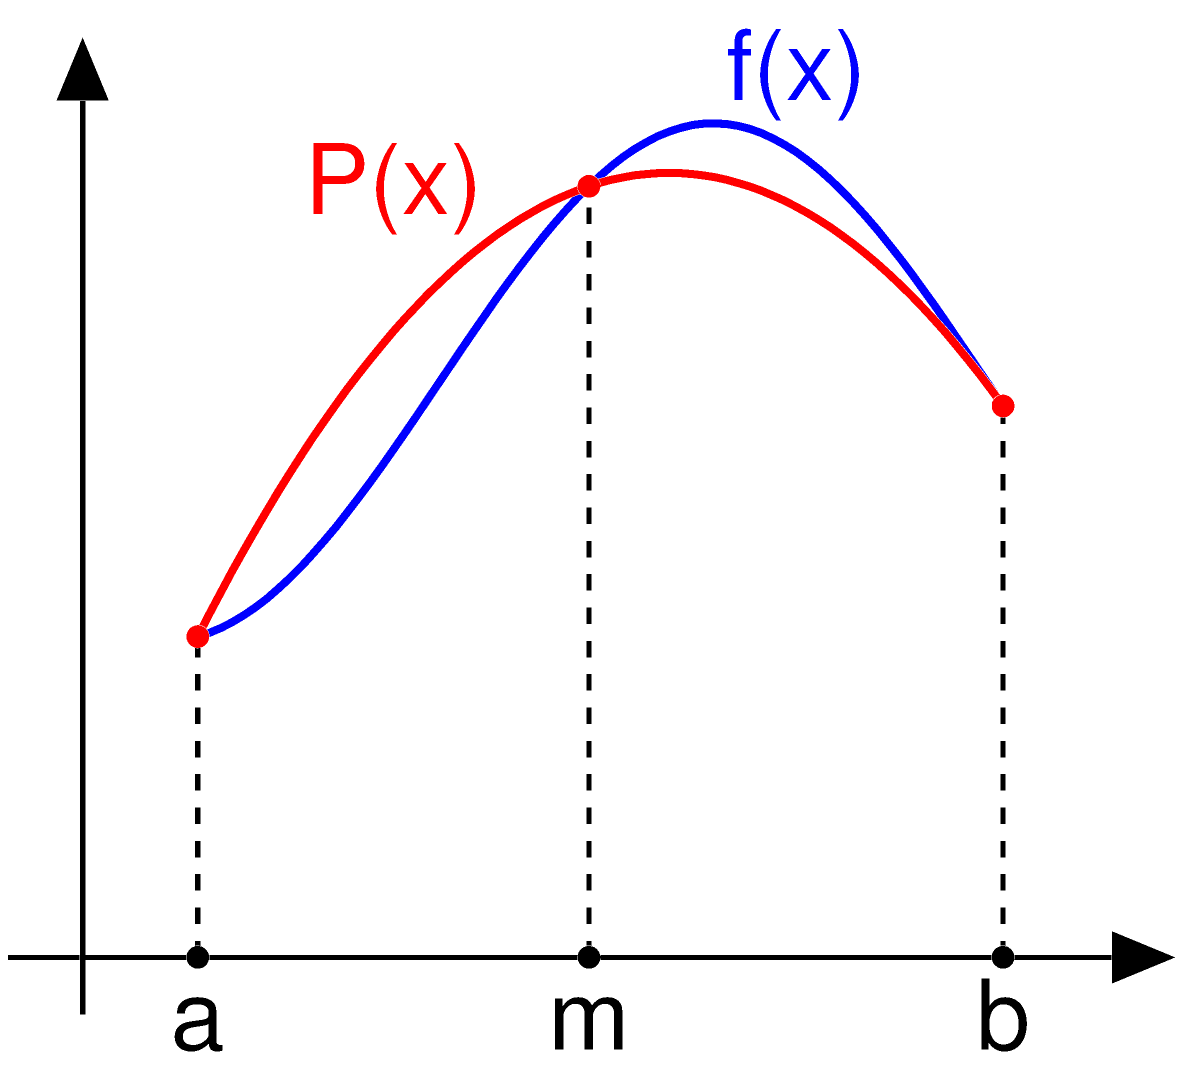
\includegraphics[width=0.6\linewidth]{Simpsons_method_illustration.png} 
\end{figure}

For example, the parabola between any two points, \((u, f(u))\) and
\((w, f(w))\) is drawn according to the formula (where
\(v=\frac{w-u}{2}\)): \begin{align*} 
p(x) = f(u) \frac{(x-v)(x-w)}{(u-v)(u-w)} +f(v) \frac{(x-u)(x-w)}{(v-u)(v-w)} + f(w) \frac{(x-u)(x-v)}{(w-u)(w-v)}
\end{align*} Then, the integral under that parabola is: \begin{align*} 
 \int_u^w p(x)dx = \frac{h}{3}(f(u) + 4(f(v)) + f(w))
\end{align*} If we imagine carrying on that calculation many times
between different points along the curve, we get \begin{align*} 
 \int_a^b f(x) dx & \approx S\\
  S &= \frac{h}{3}(f(x_0) + 4f(x_1) + 2f(x_2) + 4f(x_3)... + 4f(x_{n-1}) + f(x_n))\\
  \text{where } h=\frac{b-a}{n}\\
\end{align*}

\begin{figure}[h!]\centering 
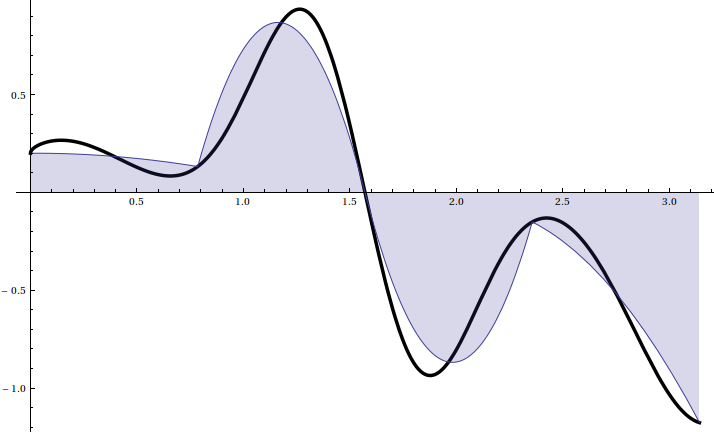
\includegraphics[width=0.6\linewidth]{simpson.png} 
\end{figure}

\section*{Create an S4 Package}
\begin{enumerate}
\item To prepare for your midterm, you will use \texttt{devtools} to create an S4 R package named \texttt{integrateIt}.

\item The package should include appropriate functions and appropriate documentation. For example, your package documentation needs to provide example usage that verifies basic functionality.

\item The package should have two classes: \texttt{Trapezoid} and \texttt{Simpson}

\item The package should have one generic: \texttt{integrateIt}

\item The package should contain at least two methods: \texttt{integrateIt}, \texttt{print}, and an optional extra credit method \texttt{tolTest}
\begin{enumerate}
\item \texttt{integrateIt} method 
\begin{enumerate}
\item Takes four arguments: a vector of values $(x)$, a vector of evaluated values $(f(x)=y)$, starting/ending values $(a,b)$, and a \textit{Rule} argument that can be either "Trapezoid" or "Simpson".
\item Have three outputs: an object of class \texttt{Trapezoid} or class \texttt{Simpson}, the values of $x$ and $y$, and the result
\item Both classes should have validation methods that include a few appropriate tests
\item you will need to create an \texttt{initialize} function for each class, which will be used internally by \texttt{integrateIt}
\end{enumerate}



\item \texttt{print} method 
\begin{enumerate}
\item A very simple print method for each class, which prints out just the integrated value (rather than all of the results)
\end{enumerate}

\end{enumerate}

\begin{enumerate}
\item Extra Credit: \texttt{tolTest} method
\begin{enumerate}
\item A \texttt{fun} (function)
\item A \texttt{tolerance} argument
\item A \texttt{rule} argument that indicates whether the Trapezoidal or Simpson's 
\item A \texttt{start} argument for the number of intervals it should start with
\item A \texttt{correct} argument that provides the correct answer for the integral
\end{enumerate}



\texttt{tolTest} should take in a function and increase the number of intervals $n$ until the answer it provides using the specified approximation is within \texttt{tolerance} of the correct answer. Use \texttt{integrate()} to do this. \texttt{tolTest} output should be
\begin{enumerate}
\item The inputs
\item The final $n$
\item The absolute error of the estimate
\end{enumerate}
\end{enumerate}



\end{enumerate}

\end{document}
